% EPC flow charts
% Author: Fabian Schuh
\documentclass{article}
\usepackage{myflowchart}

\begin{document}

\begin{tikzpicture}

\begin{scope}[node distance=5mm and 5mm]

\node [ item=4](a) at (1,1) {%
            \textbf{weekly routine}
            \nodepart[text width = 8.2cm]{two}
            \begin{enumerate}
            	\item arrange for collected readings from bloggers to update essay post.
             	\item admire, find and fix any typo or mistake.
            	\item expand some posts, ex. the csgo post.
            	\item look up collected volcab and write post.(四五月有不少還沒查的)
            	\item still need to close out DIY post.
           \end{enumerate}
           \nodepart{three}\textbf{特色}
	\nodepart[text width = 8.2cm]{four}
            \begin{enumerate}
            	\item 使用LYX與SW,高度自動化產生django-compatible html(省下很多細微瑣碎步驟)。
            	\item 讓SW與LYX產生的網頁能夠正確顯示。如SW export links時有點問題,要記錄下可行步驟,並嘗試自動化。
           \end{enumerate}
            };


	\node [above right = of a, align = center, anchor = south] (title){\parbox[c][][c]{3.2cm}{\Huge website}\parbox[c][][c]{0.15\textwidth}{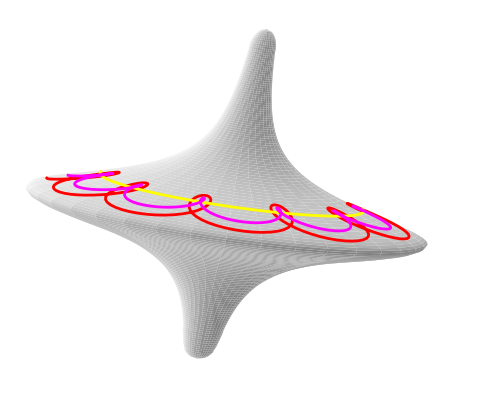
\includegraphics[width=0.15\textwidth]{../../figs/logo_June27_2016.png}}\parbox[c][][c]{3.6cm}{\Huge planning}};


\node [ item=2, below right = of title.south, anchor = north west](small) {%
            \textbf{重點步驟}
            \nodepart[text width = 8.2cm]{two}
            \begin{enumerate}
            	\item when generating html files from LYX for the website, a few steps need to be followed in order to make it work. Most webpages on this site are generated by LYX, even the django-compatible html pages. In order to make this work a few things has to be followed during the LYX exporting process.
            	\item To generate webpost that has the head banner, after LYX html export, run LYX2HTML\_header\_replace.py
            	\item To generate webpost that has Scribd pdf preview embed code, after LYX html export, run LYX2HTML\_str\_replace.py
           \end{enumerate}
            };

\node [ wideitem=2, below right = of a, anchor = north](LYX) {%
            \textbf{creating posts utilizing LYX}
            \nodepart[text width = 16.5cm, align = left]{two}Five types of posts can be generated after the function of LYX's HTML export:
            \begin{enumerate}
            	\item normal
            	\item 若有scribd pdf preview embeded code,跑LYX2HTML\_replace\_str.py。
		\item 若要加入本工作室設計的banner header(網頁上方的logo加標題加一條線),跑LYX2HTML\_banner\_replace.py。
		\item 若有數學公式,在使用LYX html export之前,要去設定converter,加上-mathjax指令,用完之後記得要把converter的-mathjax指令移除,也就是設定回原本狀態。這步驟有點麻煩,如何改進?
		\item 若輸出的html檔包含有需要被伺服的圖檔,則LYX插入圖片時可按照以下整理好的流程
		\begin{enumerate}
			\item 將所需圖片先複製到與LYX檔案相同位置(在myblogpost資料夾那邊,不是template那邊),名為static的資料夾下。
			\item 在LYX檔中從上述資料夾插入圖片
			\item 執行LYX html export功能,此功能經過我們更改,檔案會自動export至template資料夾。這樣圖片也會copy到那邊的static資料夾。
			\item 運行django指令collectstatic收集所有template資料夾中要被伺服的眾多static資料夾。
			\item (若有信心沒有bug可省略)設定debug=true(這樣本地端static資料夾才會被伺服),運行django本地端測試local test server。沒問題設定回debug=false。
			\item git commit時記得要track圖片!!!git push to deploy.
		\end{enumerate}
           \end{enumerate}
            };

\end{scope}
\end{tikzpicture}
\end{document}
